\chapter{Analýza}
\section{Funkční speficikace}
Framework musí umožňovat uživateli vytvářet a dále pracovat s vytvořenými komponentami. Komponenty budou procházet určitým životním cyklem. Kromě samotných komponent musí framework poskytovat i dodatečné funkcionality, které jsou spojeny se získáváním dat, jejich propagací na klienta, zabezpečení, organizací komponent, lokalizací a skinováním komponent.
\subsection{Funkční požadavky}
Z dosavadního popisu problému byly vytvořeny následující požadavky na systém.
\begin{itemize}
\item Framework bude umožňovat generovat metadata objektů, na základě kterých budou generovány komponenty.
\item Framework bude umožňovat vygenerovat formulář nebo tabulku na základě dat získaných ze serveru.
\item Framework bude umožňovat získat data ze serveru.
\item Framework bude umožňovat naplnit formulář i tabulku daty.
\item Framework bude umožňovat odeslat data z formuláře zpět na server.
\item Framework bude umožňovat používat lokalizační resource bundly.
\item Framework bude umožňovat validaci dat na základě metadat, která obdržel od serveru.
\item Framework bude umožňovat klientovi překrýt chybové validační hlášky.
\item Framework bude umožňovat skinovatelnost.
\item Framework bude umožňovat specifikovat zdroje ve formátu xml.
\item Framework bude umožňovat vytvářet vstupní pole, combo boxy, výstupní pole, textarea, checkboxy, option buttony.
\item Framework bude umožňovat vkládat do formulářových polí texty, čísla a datumy.
\item Framework bude umožňovat generování readonly komponent. 
\end{itemize} 
Z požadavků vyplívá, že framework bude umožňovat získání definici dat na serveru a poté je distribuuje koncovému uživateli. Koncový uživatel tedy nebude potřebovat znát obejkty, s kterými pracuje. Toto zaručí pružnou reakci na změnu dat a generování aktuálních formuláří či tabulek. 
\subsection{Nefunkční požadavky}
\begin{itemize}
\item Framework generovat metadata, která nebudou závislá na platformě.
\end{itemize} 
\section{Popis architektury a komunikace}
Jak již bylo uvedeno, tak je definice objektů, na základě kterých se budou vytvářet komponenty, generována na serverové straně. Klient tedy komunikuje se serverem a vyžádá si tyto definice. Dále je potřeba definice na klientovi zpracovat. Definice budou platformově nezávislé. Budou tedy popisovat data v obecné formě, aby bylo možné generovat formuláře a tabulky nezávisle na platformě, jazyku a technologii. Referenční implementace bude napsána v jazyce Java s využitím komponentového frameworku Swing. Data, která jsou zasílány ze serveru na klientovi by neměli ovlivňovat ostatní klienty, kteří framework nepoužívají. 

Business proces, který zachycuje generování formuláře včetně validace a odeslání je zachycen na obrázku \ref{img:businessModel}. Uživatel nejprve specifikuje zdroje, které bude klient využívat. Rozeznáváme následující zdroje:
\begin{enumerate}
\item Zdroj s metadaty, které definují komponentu.
\item Zdroj s daty, které budou v komponentech zobrazeny.
\item Zdroj, na který budou data odeslána.
\end{enumerate}
Následně je vygenerována komponenta na základě metadat. V případě, že byl specifikován zdroj s daty, tak klientská část aplikace požádá server o tato data a vloží je do předpřipravené komponenty. Pokud datový zdroj specifikován není, tak zůstane komponenta bez konkrétního obsahu. Komponenta je nyní připravena a uživatel s ní může pracovat. V případě, že uživatel chce odeslat data na server a specifikoval zdroj, na který budou data odeslána, pak framework provede validaci dat. Pokud je validace dat úspěšná, tak se na základě metadat sestaví objekt, který je naplněn daty z aktuálního formuláře a odeslán na server. Server zpracuje request a vrátí klientovi odpověď. Na základě této odpovědi může uživatel dále upravovat formulář či s ním pracovat.

\subsection{Metadata}
Metadata jsou data, která popisují jiná data. Framework, který je popsán v této práci generuje na serverové straně metadata a zasílá je na klienta, který na jejich základě sestaví komponenty a poté je s nimi schopný pracovat. Klient musí být schopný zpětně sestavit data a odeslat je na server. Klient využívá klientskou část frameworku a server serverovou část. Z hlediska implementace je důležité, aby objekty nesoucí informace o metadatech stejné a bylo možné provést na klientovi generování na základě těchto dat.
Následující doménový model znázorňuje popis definic objektu, který je vytvořen po inspekci zadaného objektu. Inspekce vytvoří XML popis, který je převeden na obecný popis, jenž lze využít ke generování dat na klientovi. Tento obecný popis je zaslán klientovi, který využívá klientskou část frameworku. Klientská část frameworku očekává tyto objekty a na jejich základě je schopná vygenerovat uživatelské rozhraní. Na obrázku \ref{img:metadataModel} je zobrazen doménový model \cite{UmlArlow}, který je použit při popisu metadat objektu. Nejedná se o doménový model frameworku, ale pouze jeho části, která je zodpovědná za reprezentaci metadat. 

\begin{figure}[h!]
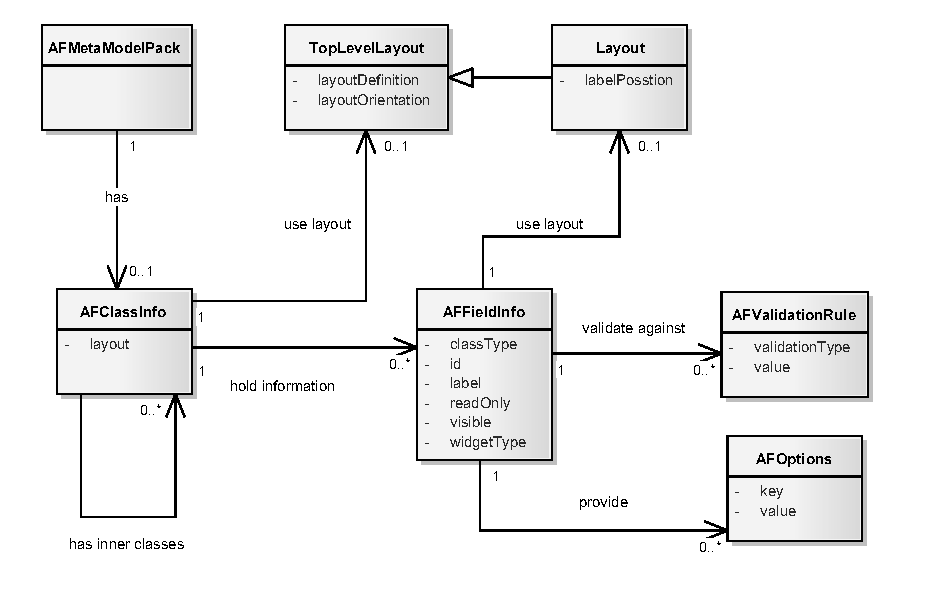
\includegraphics{images/domainModel}
\caption{Doménový model obejktů obsahující metadat o objektu, nad kterým byla provedena inspekce}
\label{img:metadataModel}
\end{figure}

\subsubsection{AFMetaModelPack}
Tato třída zapouzdřuje informace, které popisují objekt, nad kterým byla prováděna inspekce. Třída rovněž slouží jako fasáda a nabízí programátorovi upravení metadat po generování. V případě serveru je toto návratový typ zdroje, na který klient přistoupí chce-li znát metadata, která zdroj poskytuje.
\subsubsection{AFClassInfo}
Tato třída udržuje informace o hlavním objektu, z kterého je vytvářena definice. Třída má dále reference na své vnitřní proměnné a své potomky. Na základě generování dat je potřeba udržet pořadí, v kterém byla nad jednotlivými komponenty prováděna inspekce. V případě inspekce dat je i reference na neprimitivní datový typ jeho proměnná. Nicméně je potřeba, aby klient byl schopný určit, že se jedná o složitý datový typ a určit jeho pořadí v aktuálním objektu, aby mohl rozhodnout na jaké pozici objekt zobrazit. Z tohoto důvodu je v této třídě proměnná classType, která určuje zdali se jedná o vnitřní třídu či primitivní datový typ.
\subsubsection{AFFieldInfo}
Tato třída je zodpovědná za poskytování detailních informací o proměnné objektu, nad kterým byla provedena inspekce. Třída udržuje název proměnné, widget, na který bude proměnná převedena, pravidla, která musí být splněna a název pod kterým, bude prezentována uživateli. Kromě těchto vlastností nese objekt také informace o tom, zdali je komponenta viditelná a zdali je pouze pro čtení.
\subsubsection{AFRule}
Každá proměnná má souhrn vlastností, které musí být splněny. Typ widgetu ještě vždy nemusí určovat datový typ komponenty. Dále neurčuje, zdali je pole povinné či nikoliv. Tento soubor vlastností je popisován v této třídě. Třída využívá ENUM, který specifikuje podporované validace. Důvodem je to, že klient musí být schopný vytvořit tyto validační pravidla a interpretovat je na komponentě svým vlastním způsobem, který je specifický pro technologii, kterou používá. Jednou z dalších výhod je validace XML, z kterého jsou pravidla vytvářena. Framework vytvoří pouze ty validační pravidla, která podporuje. Klient poté musí podporovaná pravidla interpretovat. 
\subsubsection{AFOptions}
Některé widgety umožňují, aby si uživatel vybral z několika předem připravených možností. Tyto možnosti musí být klientovi prezentovány. Tato třída udržuje informace o možnostech výběru v dané komponentě. Proměnná klíč je hodnota, která bude odeslána zpět na server a proměnná value je hodnota, která bude zobrazena klientovi. Tímto způsobem lze klientovi zobrazit jakýkoliv text, který bude zpětně mapován na jeho skutečnou hodnotu. Kromě textu lze samozřejmě zobrazit čísla či hodnoty výčtových typů.

\subsection{Server}
Server je zařízení či software, který umožňuje zpracovat požadavky od klientů a na jejich základě vytvořit odpověď. Server tedy poskytuje svým klientům určitý typ obsahu. Způsob a původ obsahu, který server poskytuje je pro klienta povětšinou neznámý. V současné době je velmi populární přístup, při kterém server získá data z vice zdrojů a poskytne je klientovi. Hovoříme o tzv mashup \cite{Tuchinda2008}. Mashup nemusí být pouze z veřejných zdrojů, lze využít i zdroje z privátních zdrojů, či lze k sestavení odpovědi využít další služby. Klient napojený na server tohoto typu nemusí mít o těchto dalších zdrojích vůbec žádnou povědomost a dotazuje se pouze vůči tomuto serveru, který zpracovává jeho požadavky. 
Klienti, kteří získávají data z veřejných, či privátních zdrojů serveru může být spousta. Mohou to být vlastní privátní aplikace, mobilní aplikace, javascriptoví klienti či další server, který pouze využívá veřejné zdroje serveru k sestavení odpovědi svým vlastním klientům. V těchto případech je potřeba zvážit způsob generování definic dat, které by mohly způsobit stávajícím klientům problémy. V ideálním případě, je tedy potřeba framework integrovat takovým způsobem aby byla zachována stávající funkcionalita a framework ji pouze rozšířil. 
Ke generování definic objektů jsou potřeba následující věci:
\begin{enumerate}
\item Objekt, jehož definice budou generovány.
\item Mapování, na základě, kterého bude rozhodnuto, o jaký typ komponenty půjde.
\item Definice komponenty včetně jejich vlastností jako jsou validace, layout a popis chování komponenty.
\item Layout, v kterém budou komponenty sestaveny.
\item Framework, který provede inspekci.
\item Framework, který bude inspekci řídit a bude interpretovat vygenerovaná data. Tento framework musí zároveň ověřit validitu jednotlivých komponent.
\end{enumerate}

Výše uvedené vlastnosti, nebudou mít vliv na změnu funkcionality. K inspekci a mapování bude využit framework AspectFaces \cite{aspectFaces}, který umožňuje na základě datových typů rozhodnout jakou komponentu využít. Definice komponent a jejich vlastností bude již v plné kompetenci vývojáře, nicméně základní komponenty a jejich chování bude předpřipraveno ve vzorovém projektu aby se vývojář mohl inspirovat.
Server využívá serverovou část.

\subsection{Klient}
Klientská část frameworku bude vytvářet komponenty na základě metadat, která obdržela od serveru. Klient nebude mít žádnou znalost o objektech, které mu server poskytuje předtím než obdrží jejich definice. Klient nicméně musí vědět, který zdroj mu poskytne relevantní definice, a který ze zdrojů mu poskytne data odpovídající těmto definiciím. Zároveň také musí vědět, na který zdroj data zpětně odeslat. Zdroj je obvykle specifikován následujícími parametry:
\begin{enumerate}
\item Adresa serveru
\item Port
\item Protokol
\item Metoda (get, post, put, delete)
\item Dodateční hlavičkové parametry například content-type
\end{enumerate}
Klient tedy bude muset vždy specifikovat tyto parametry. Z hlediska použitelnosti je vhodné mít tyto specifikace v XML souboru, který bude umět klient jednoduše načíst. Pro usnadnění bude načítání provádět framework.  Ukázka je na obrázku \ref{code:xmlSource}. V ukázkovém příkladu je specifikován zdroj z metadaty, který je vždy povinný. Zdroj se nachází na adrese\\ http://localhost:8080/AFServer/rest/users/loginForm. Zdroj s daty není specifikován, což způsobí, že ve formuláři nebudou žádná data. Formulář bude možné odeslat na adresu http://localhost:8080/AFServer/rest/users/login. Zdroj má identifikátor loginForm. V jednom XML dokumentu lze mít více zdrojů. Data to konkrétního zdroje lze vkládat pomocí EL. V hlavičce může být 0 až N parametrů, přičemž každý parameter musí být uveden ve stejném formátu jako je znázorněno na obrázku \ref{code:xmlSource}. Obdobný způsob se využívá v JavaEE aplikací v deskriptoru web.xml. Klient umí sestavit request na základě tohoto popisu a interpretovat odpověď od serveru. Není tedy nutné aby uživatel implementoval třídy, které se zvládnout připojit na server a získat data.

\begin{lstlisting}[caption=Ukázka XML specifikace zdrojů,
  label=code:xmlSource]
<?xml version="1.0" encoding="UTF-8"?>
<connectionRoot xmlns:xsi="http://www.w3.org/2001/XMLSchema-instance">
	<connection id="loginForm">
		<metaModel>
			<endPoint>localhost</endPoint>
			<endPointParameters>/AFServer/rest/users/loginForm</endPointParameters>
			<protocol>http</protocol>
			<port>8080</port>
			<header-param>
				<param>content-type</param>
				<value>Application/Json</value>
			</header-param>
		</metaModel>
		<send>
			<endPoint>localhost</endPoint>
			<endPointParameters>/AFServer/rest/users/login</endPointParameters>
			<protocol>http</protocol>
			<port>8080</port>
			<method>post</method>
			<header-param>
				<param>content-type</param>
				<value>Application/Json</value>
			</header-param>
		</send>
	</connection>
</connectionRoot>
\end{lstlisting}

Je patrné, že klient je schopný získat definice formulářů či tabulek, naplnit je daty a poté zpět odeslat na server. Důvodem, proč je klient schopný generovat formuláře na základě definice ze serveru je ten, že klient pracuje se stejnými objekty, které popisují metadata, jako server. Prozatím je k dispozici pouze strohý popis dat. Klientská část musí nyní rozhodnout jak data interpretovat, jak s nimi pracovat, jakým způsobem je validovat a jak je znovu sestavit a odeslat na server. Důležitým prvkem je i způsob uspořádání jednotlivých prvků, jejich velikosti, barvy a texty.

Využití frameworku by obdobně jako v případě serveru nemělo mít vliv na stávající použití aplikace. V případě referenčního řešení ve Swingu generuje klient JPanel, který lze vkládat do dalších panelů a vývojář tak není nikterak omezen co se týče stávající aplikace. 

\begin{figure}[h!]
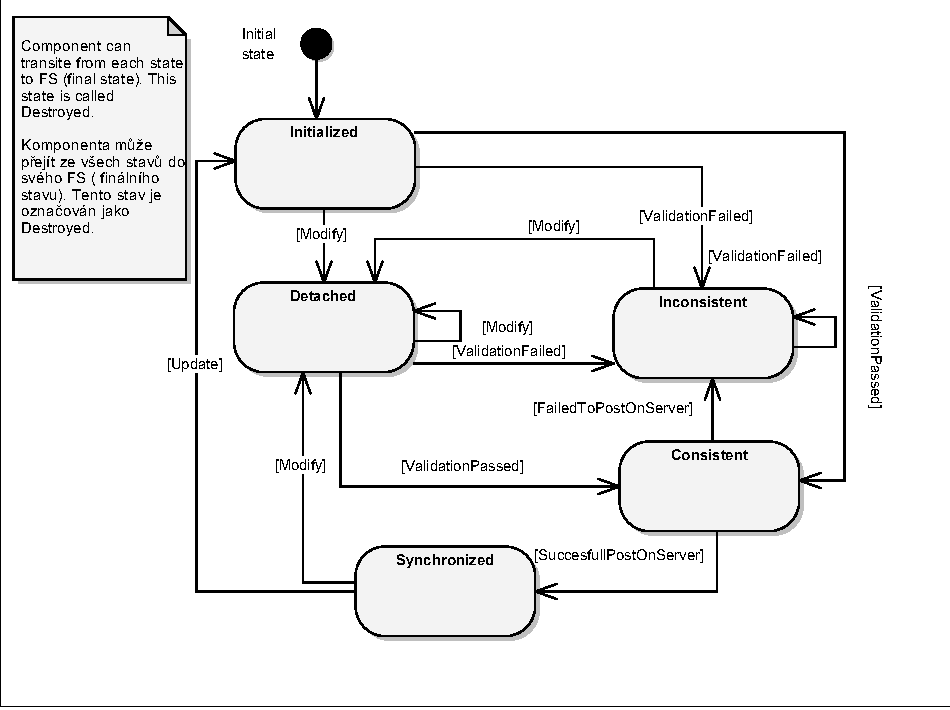
\includegraphics{images/formLifecCycle}
\caption{Životní cyklus formuláře}
\label{img:formLifeCycle}
\end{figure}

\subsection{Životní cyklus formuláře}
Formulář, jako každá komponenta, má svůj životní cyklus. Jeho stavy jsou znázorněny na obrázku \ref{img:formLifeCycle}. Formulář je po vygenerování a po naplnění daty v inicializačním stavu. V tomto stavu může být komponenta nevalidní, neboť data, která obdržela nemusí splňovat požadované validace. K této situaci může dojít, je-li například přidána nová proměná do datového modelu. Toto přidání obvykle probíhá tak, že se v koncové databázy, pokud jí software má, přidá políčko a nastaví se mu defaultní hodnota pro již existující data, či je hodnota null. Nicméně v definici může být pole označeno jako povinné, avšak ve formuláři nemusí být pole vyplněno, což způsobí, že jsou data nevalidní, byť uživatel ve formuláři data nezměnil. Komponenta se pak přepne do stavu Inconsistent. V případě modifikace dat se komponenta dostává do stavu Detached. Tento stav značí, že byla data změněná. Pokud uživatel data stále mění, pak komponenta zůstává v tomto stavu. Ze stavu Detached přechází komponenta v případě úspěšné validace do stavu Consistent. V případě neúspěšné validace se komponenta dostane do stavu Inconsistent. Z tohoto stavu lze přejít pouze do dvou stavů jedním z ních je stav Detached. Do tohoto stavu lze přejít pokud uživatel změní data ve formuláři. Komponenta může také zůstat ve stavu Inconsistent, pokud uživatel data nezmění a zkusí provést validaci znovu a tato validace opět selže. Konzistentní stav značí, že je komponenta připravená k odeslání dat na server. Pokud odeslání dat selže je komponenta přepnuta do stavu Inconsistent, v případě úspěšného odeslání dat, je komponenta přepnuta do stavu Synchronized. Ze stavu synchronized lze přejít do stavu Initialized, pokud jsou data znovu načtena ze serveru a do stavu Detached, pokud jsou data upravena uživatelem.

\section{Případy užití}
Případy užití a jejich scénáře \cite{UmlArlow} specifikují chování systému. V této práci lze nahlížet na případy užití ze dvou stran. První z nich je koncový uživatel nebo-li vývojář, který framework využívá. Druhým z nich je samotný framework, který provádí akce, aby splnil úkol, který mu uživatel uložil. V této sekci se zaměříme na případy užití koncového uživatel, které specifikují použití frameworku. Na obrázku \ref{img:useCase} jsou zachyceny všechny tyto případy užití. Pro ukázku detailně rozebereme případ užítí na obrázku \ref{img:useCaseSmall}. Na tomto případu je znázorněno odeslání dat z vygenerovaného formuláře zpět na server. Součástí je samozřejmě validace zadaných dat a jejich zpětné sestavení, neboť formulář byl vytvořen na základě metadat a klient tedy zná pouze strukturu objektu popsanou těmito metadaty. 
\begin{figure}[h!]
\begin{center}
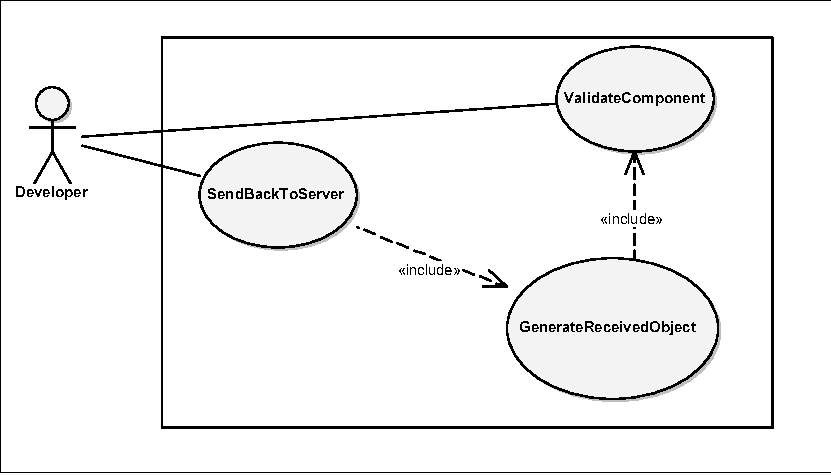
\includegraphics{images/useCaseSmall}
\caption{Část případů užití znázorňující odeslání dat na server z vygenerovaného formuláře}
\label{img:useCaseSmall}
\end{center}
\end{figure}
\subsubsection{Validace komponenty}
Tento případ užití je znázorněn na obrázku \ref{img:useCaseSmall} a jmenuje se ValidateComponent.

Případ užití: Validace komponenty\\
ID: 1\\
Popis: 
Uživatel využívá framework ke generování formulářů. Hlavním úkolem formuláře je možnost vkládat či upravovat data a odesílat je zpět na server. Před odesláním dat na server musí být provedena validace, aby se zajistilo, že bude formát dat serveru vyhovovat a bude umět s daty pracovat.
\\
Aktér: Uživatel\\
Vstupní podmínky:
\begin{enumerate}
\item Formulář musí být sestaven na základě metadat a framework musí znát formulář s kterým chce pracovat.
\end{enumerate}
Scénář:
\begin{enumerate}
\item Případ užití začíná obdržením požadavku od uživatele žadající validaci dat.
\item Systém vyhledá pole k validaci.
\item Dokud existují pole k validaci pak:
\begin{enumerate}
\item Systém získá konkrétní pole k validaci.
\item Systém určí typ komponenty a požádá builder, který ji sestavil o data.
\item Dokud existuje validace, která zatím nebylo na poli vykonána pak:
\begin{enumerate}
\item Systém požádá validátor o validaci.
\item Pokud validace selže pak:
\begin{enumerate}
\item Systém ukončí validování tohoto pole a zobrazí u něj chybovou validační hlášku.
\end{enumerate}
\end{enumerate}
\end{enumerate}
\end{enumerate}

Případ užití: Sestavení dat\\
ID: 2\\
Popis: 
Uživatel využívá framework ke generování formulářů. Hlavním úkolem formuláře je možnost vkládat či upravovat data a odesílat je zpět na server. Před odesláním dat na server musí být tyto data zpětně sestaveny, aby s nimi server dokázal pracovat.
\\
Aktér: Uživatel\\
Vstupní podmínky:
\begin{enumerate}
\item Formulář musí být sestaven na základě metadat a framework musí znát formulář s kterým chce pracovat. Framework musí znát formát dat, které server očekává.
\end{enumerate}
Scénář:
\begin{enumerate}
\item Případ užití začíná obdržením požadavku od uživatele žadající sestavení dat z formuláře.
\item Zahrnout(Validace komponenty).
\item Pokud validace dopadla úspěšně pak:
\begin{enumerate}
\item Systém získá pole, která budou odeslána.
\item Pokud exsituje pole, které ještě nebylo transformováno pak:
\begin{enumerate}
\item Systém určí typ komponenty a požádá builder, který ji sestavil o data.
\item Systém určí název proměnné a třídu, do které patří a nastaví ji data.
\end {enumerate}
\item Systém na základě formátu dat, které server očekává rozhodne v jakém formátu data zaslat a převede je na daný formát.
\end{enumerate}
\end{enumerate}

Výstupní podmínka:
\begin{enumerate}
\item Data ve formuláři byla převedena na objekt, s kterým umí server pracovat.
\end{enumerate}

Případ užití: Odeslání dat\\
ID: 3\\
Popis: 
Uživatel využívá framework ke generování formulářů. Hlavním úkolem formuláře je možnost vkládat či upravovat data a odesílat je zpět na server. Před odesláním dat na server musí být tyto data zpětně sestaveny, aby s nimi server dokázal pracovat a musí splnit validační kritería
\\
Aktér: Uživatel\\
Vstupní podmínky:
\begin{enumerate}
\item Formulář musí být sestaven na základě metadat a framework musí znát formulář s kterým chce pracovat. Framework musí znát zdroj, na který mají být data odeslána a všechny potřebné informace, které zdroj vyžaduje.
\end{enumerate}
Scénář:
\begin{enumerate}
\item Případ užití začíná obdržením požadavku od uživatele žadající odeslání formuláře na server.
\item Zahrnout(Validace komponenty).
\item Zahrnout(Sestavení dat)
\item Dokud je validace či sestavení dat neúspěšné pak:
\begin{enumerate}
\item Systém zobrazí chybové hlášky a určí, u kterých poli nastala chyba
\item Uživatel chybu opraví a požádá systém o opětovnou validaci a sestavení dat.
\end{enumerate}
\item Systém vytvoří připojení na specifikovaný zdroj a odešle data.
\item Pokud odeslání selhalo pak:
\begin{enumerate}
\item Systém zobrazí chybovou hlášku, že nebylo možné data odeslat včetně odpovědi od serveru, je-li nějaká.
\end{enumerate}
\end{enumerate}

Výstupní podmínka:
\begin{enumerate}
\item Data byla odeslána.
\end{enumerate}


\section{Omezení frameworku}
Existují určité možnosti, které nebudou ve frameworku podporovány. V následujícím přehledu budou představeny nepodporované vlastnosti frameworku v aktuální verzi.
\begin{enumerate}
\item Inspekce datových proměnných typu List a Array
\item Získávání dat ve formátu XML. Framework plně podporuje JSON.
\item Customizace jednotlivých polí. Framework podporuje customizaci formuláře a všech jeho polí, nicméně nedisponuje možností přizpůsobovat jednotlivá pole.
\item Odesílání dat a validace dat v tabulce. Tabulka je v této verzi pouze readonly, data tedy nemá smyls odesílat zpět na server.
\item Framework vyžaduje ke své funkčnosti jak serverovou tak klientskou stranu. V případě, že klientské straně chybí serverová strana, tak je framework nefunkční. V případě, že serverové straně chybí klientská strana, tak je serverová strana stále schopná vytvářet definice dat.
\item Klientská strana zobrazuje pouze ta data, která obdržela od serveru, nelze vytvářet automatický Mashup na klientovi. Nicméně klient může generovaný formulář umístit mezi jiné komponenty.
\item Klientská strana nedokáže sestavit objekt, který získala z metadat do takové míry aby z něj byla schopná vytvořit instanci. Nebo-li klientská strana si neudržuje konkrétní objekt, který obdržela, pouze jeho popis.
\item Serverová část využívá k automatické inspekci framework. Bez tohoto frameworku není možné inspekci provést, nicméně uživatel si může definovat svou vlastní definici bez nutnosti inspekce dat.
\end{enumerate}

\section{Uživatelé a zabezpečení}
Téměř každá aplikace využívá způsob, při kterém se uživatel autentizuje a aplikace mu na základě jeho rolí přidělí oprávnění. V případě využití bezestavového protokolu, jakým REST je lze posílat informace o uživateli v hlavičce requestu. Tyto informace mohou být samozřejmě zašifrované. Framework podporuje vkládání libovolných informací do hlavičky requestu. Klient si také může zvolit zdali bude využívat http či https protokol. Velmi rozšířenou možností je využitý Oauth. Jednou z možností, je vložení parametrů do hlavičky či do adresy. Vkládání dynamických adres či proměných do hlavičky requestu framework podporuje. 

Druhou části jsou uživatelské role, na základě kterých se generuje uživatelské rozhranní. Serverová část využívá framework AspectFaces \cite{aspectFaces}, který podporuje uživatelské role v systému. Je jen na programátorovi, jaký framework na autentizaci a autorizace na straně serveru použije. Jednou z možností je například napsat si vlastni interceptor, který určí o jakého uživatele se jedná, přiřadí mu roli v systému, na základě které se mu zobrazí konkrétní obsah. Server při generování metadat může využít různé mapovací soubory na základě uživatelské role. Specifikace tohoto chování je opět v plné kompetenci uživatele.
\section{Použité technologie}
V následující sekci jsou rozebrány použité technologie. Kromě samotného frameworku je součástí práce i ukázkový projekt na platformě JavaEE.
\subsection{Java SE - Swing}
Klientská část frameworku je schopná vygenerovat formuláře či tabulky a naplnit je daty a data odeslat. Klientská část je přizpůsobena frameworku Swing. Důvodem je, že vývoj Swingové aplikace je rychlý a Swing zná velké množství vývojářů, kteří si framework mohou jednoduše otestovat. Nicméně metadata, která server generuje lze interpretovat v jakékoliv technologii. Swing je knihovna grafických a uživatelských prvků. Poskytuje komponenty, layouty, actionListenery, okna, dialogová okna a další prvky, pomocí kterých lze vytvářet interaktvní aplikace.
\subsection{Java EE}
Java EE je platforma sloužící k vývoji enterprise aplikací. V současné době je oblíbená jak u velkých tak u menších korporací. Java EE přináší podporu pro Restové služby, JFS, JSP, EJB, databázové frameworky, anotace  a další komponenty. Aplikace v Java EE se obvykle nasazuje na aplikační server. Aplikační servery mohou být v cloudu a podílet se společně na zpracování requestů. Důvodem využítí této platformy je fakt, že klient vytváří requesty vůči serveru a server tato data zpracovává. Je vhodné mít na serveru platformu, která je ověřená a má potenciál ke zpracování těchto requestů. V této práci generujeme data pomocí restového rozhranní a Java EE splňuje specifikaci, které se tohoto rozhranní týká. 
\subsection{AspectFaces}
AspectFaces je framework, který umí provádět inspekci nad zadanými obejkty a na základě datových typů a dalších parametrů rozhodovat o to, jaká komponenta se použije pro konkrétní datový typ. Framework využívá AspectFaces k tomu, aby provedl toto mapování a sestavil popis uživatelského rozhranní. Hlavním důvodem využití tohoto frameworku je fakt, že je distribuován jako open source pod licencí LGPL v3 a že lze využít jeho funkcionalitu ke statické inspekci dat. Tato inspekce je již odladěna a není tedy důvod psát znovu již vynalezenou věc. 
\subsection{Ukázkový projekt}
Ukázkový projekt demonstruje použití frameworku. Skládá se ze dvou částí. Klientské a serverové. Klientská část využívá pouze Swing. Serverová část je mnohem sofistikovanější a využívá aktuální technologie. Ukázkový projekt zde znázorňuje použítí frameworku a jeho omezení. Ukázkový projekt je koncipován, tak aby ho bylo možné nasadit bez nutnosti dodatečného nastavení.
\subsubsection{Glassfish}
GlassFish \cite{glassfish} je open source aplikační server, jedná se o certifikovaný server JavaEE. Umožňuje clustering, monitoring, podporu EJB, REST a JDBC. Architektura jádra je založena na frameworku OSGI, který umožňuje vzdáleně přidávat, startovat či ukončovat komponenty bez nutnosti restartování celého serveru. Důvodem proč je Glassfish využit na tomto projektu je čistě demonstrativní. Nicméně, každý aplikační server má svá specifika, a proto je ukázková aplikace odladěna právě pro GlassFish. Jak již bylo zmíněno Glassfish distribuje vestavěnou podporou pro Rest a umožňuje použití Derby DB v režimu in memory bez nutnosti speciálního nastavení.
\subsubsection{RestEasy}
Jedná se o framework, pomocí kterého lze vytvářet RESTful aplikace. Tento framework může běžet v libovolném servletovém kontajneru. Framework podporuje například JSON, XML serializace objektů, EJB a je splňuje JAX-RS implementaci. Tvorba aplikací s restovým rozhranním je tak díky tomuto frameworku mnohem jednodušší a vývoj je rychlejší. 
\subsubsection{EJB}
Enterprise JavaBeans \cite{javaEETutorial} jsou serverově orientované komponenty, které zapouzdřují business logiku a přístup do databáze. Jsou spravovány v rámci serverového kontejneru, který zajišťuje jejich vytvoření i odstranění z paměti. EJB mohou být různých typů.
\begin{itemize}
\item Stateless
\item Statefull
\item Singleton
\end{itemize}
Jak již bylo zmíněno, o jejich správu se stará serverový kontejner, nemusíme tedy řešit problémy spojené s vytvořením a destrukcí singletonu\cite{gamma}. Mezi hlavní výhody EJB patří transakční zpracování, zajištění systémových služeb a bezpečnostní autorizace. Abychom definovali či~získali přístup k těmto třídám, používáme anotace, které jsou velmi dobře čitelné a~srozumitelné.
\subsection{Derby DB}
V ukázkovém projektu je potřeba data ukládat do databáze. Při vytváření byl kladen důraz na to, aby noví uživatelé nemuseli v konfiguračních souborech specifikovat nastavení a mohli ukázkový projekt ihned nasadit a vyzkoušet. Z tohoto důvode je využita light databáze Derby. Ukázkový projekt ji využívá v in memory módu, což znamená, že budou data po zastavení serveru ztracena. Spolu s Derby DB využívá ukázkový projekt ORM s defaultním nastavením na create jsou v čisté databázy vytvořeny požadované tabulky, které odráží definice objektů, jenž jsou anotované jako entity. Další výhodou je možnost využít anotací k nastavení validací přímo na databázy. Toto validace pak mohou být využity při inspekci dat a na jejich základě mohou být vytvořeny validace, či konkrétní komponenty.
